\documentclass[border=2pt]{standalone}
\usepackage[T1]{fontenc}
\usepackage{lmodern,amsmath,amssymb,tikz}
\usetikzlibrary{arrows.meta}
\definecolor{direct}{RGB}{37,82,156}
\definecolor{spoke}{RGB}{100,100,108}
\definecolor{src}{RGB}{195,80,15}
\tikzset{
  v/.style={circle,fill=black,inner sep=1.35pt},
  ins/.style={rectangle,draw=black,fill=white,line width=0.6pt,minimum size=4.0pt,inner sep=0pt},
  intedge/.style={black,line width=1.15pt},
  spk/.style={spoke,line width=0.62pt},
  mk/.style={direct,line width=1.05pt},
  sarr/.style={-{Stealth[length=1.25mm,width=0.95mm]},src,line width=0.65pt}
}
\begin{document}
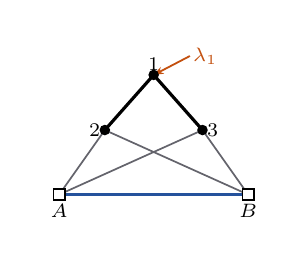
\begin{tikzpicture}[x=1cm,y=1cm,font=\scriptsize]
\path[use as bounding box] (-0.40,-0.46) rectangle (2.80,2.12);
\coordinate (A) at (0,0);
\coordinate (B) at (2.4,0);
\draw[mk] (A)--(B);

\coordinate (v1) at (1.20,1.52);
\coordinate (v2) at (0.58,0.82);
\coordinate (v3) at (1.82,0.82);
\draw[spk] (v2)--(A); \draw[spk] (v2)--(B);
\draw[spk] (v3)--(A); \draw[spk] (v3)--(B);
\draw[intedge] (v1)--(v2); \draw[intedge] (v1)--(v3);
\draw[sarr] (1.66,1.76)--(v1); \node[src,right,inner sep=1pt] at (1.66,1.76) {$\lambda_1$};
\foreach \p in {v1,v2,v3}{\node[v] at (\p) {};}
\node[above,inner sep=1.5pt] at (v1) {$1$};
\node[left,inner sep=1.5pt] at (v2) {$2$};
\node[right,inner sep=1.5pt] at (v3) {$3$};

\node[ins] at (A) {}; \node[below,inner sep=1pt] at (0,-0.08) {$A$};
\node[ins] at (B) {}; \node[below,inner sep=1pt] at (2.4,-0.08) {$B$};
\end{tikzpicture}
\end{document}
